\documentclass{article}

% if you need to pass options to natbib, use, e.g.:
\PassOptionsToPackage{numbers, compress}{natbib}
% before loading neurips_2021

% ready for submission
\usepackage[final]{neurips_2021}

% to compile a preprint version, e.g., for submission to arXiv, add add the
% [preprint] option:
%     \usepackage[preprint]{neurips_2021}

% to compile a camera-ready version, add the [final] option, e.g.:
     %\usepackage[final]{neurips_2021}

% to avoid loading the natbib package, add option nonatbib:
%\usepackage[nonatbib]{neurips_2021}

\usepackage[utf8]{inputenc} % allow utf-8 input
\usepackage[T1]{fontenc}    % use 8-bit T1 fonts
\usepackage{hyperref}       % hyperlinks
\usepackage{url}            % simple URL typesetting
\usepackage{booktabs}       % professional-quality tables
\usepackage{amsfonts}       % blackboard math symbols
\usepackage{nicefrac}       % compact symbols for 1/2, etc.
\usepackage{microtype}      % microtypography
\usepackage{xcolor}         % colors

\usepackage{amsmath,amssymb,dsfont,color,bm,mathtools,enumitem}
\mathtoolsset{showonlyrefs}
\usepackage{amsthm}
\usepackage{subcaption}

\newtheorem{thm}{Theorem}
\newtheorem{lem}{Lemma}
\newtheorem{prop}{Proposition}
\newtheorem{pro}{Property}
\newtheorem{cor}{Corollary}

\theoremstyle{definition}
\newtheorem{defn}{Definition}
\newtheorem{assumption}{Assumption}
\newtheorem{example}{Example}
\newtheorem{rmk}{Remark}

% If you use BibTeX in apalike style, activate the following line:
%\bibliographystyle{apalike}
\input macros.tex
\usepackage{mathrsfs}  
\def\caliB{\mathscr{B}}

\title{Nonparametric tensor estimation with \\
unknown permutations}

% The \author macro works with any number of authors. There are two commands
% used to separate the names and addresses of multiple authors: \And and \AND.
%
% Using \And between authors leaves it to LaTeX to determine where to break the
% lines. Using \AND forces a line break at that point. So, if LaTeX puts 3 of 4
% authors names on the first line, and the last on the second line, try using
% \AND instead of \And before the third author name.

\author{%
  Chanwoo Lee \\
  Department of Statistics\\
  University of Wisconsin-Madison\\
  \texttt{chanwoo.lee@wisc.edu} \\
  % examples of more authors
   \And
   Miaoyan Wang \\
   Department of Statistics \\
   University of Wisconsin-Madison \\
   \texttt{miaoyan.wang@wisc.edu} \\
  % \AND
  % Coauthor \\
  % Affiliation \\
  % Address \\
  % \texttt{email} \\
  % \And
  % Coauthor \\
  % Affiliation \\
  % Address \\
  % \texttt{email} \\
  % \And
  % Coauthor \\
  % Affiliation \\
  % Address \\
  % \texttt{email} \\
}

\begin{document}

\maketitle

\begin{abstract}
 We consider the problem of structured tensor denoising in the presence of unknown permutations. Such data problems arise commonly in recommendation system, neuroimaging, community detection, and multiway comparison applications. Here, we develop a general family of smooth tensors up to arbitrarily index permutations; the model incorporates the popular block models and graphon models. We show that a constrained least-squares estimate in the block-wise polynomial family achieves the minimax error bound. A phase transition phenomenon is revealed with respect to the smoothness threshold needed for optimal recovery. In particular, we find that a polynomial of degree of $m(m-1)/2$ is sufficient for accurate recovery of order-$m$ tensors, whereas higher degree exhibits no further benefits.  Furthermore, we provide an efficient polynomial-time Borda count algorithm that provably achieves optimal rate under monotonicity assumptions. The efficacy of our procedure is demonstrated through both simulations and Chicago crime date analysis. 
\end{abstract}
\vspace{-.3cm}
\section{Introduction}\label{sec:int}
\vspace{-.3cm}
Higher-order tensor datasets are rising ubiquitously in modern data science applications, for instance, recommendation systems \citep{baltrunas2011incarmusic}, social networks \citep{nickel2011three},
genomics \citep{wang2019common}, and neuroimaging \citep{zhou2013tensor}.
Tensor structure provides effective representation of data that classical vector- and matrix-based methods fail to capture. 
One example is music recommendation system that records ratings of songs from users on different contexts \citep{baltrunas2011incarmusic}. This three-way tensor of user$\times$song$\times$context allows us to investigate interaction of users and songs under a context-specific manner.
Another example is network analysis that studies the connection pattern among nodes.  Pairwise interactions are often insufficient to capture the complex relationships, whereas multi-way interactions improve understanding the networks in molecular system \citep{Michoel2012AlignmentAI} and computer vision \citep{Agarwal2006HigherOL}. In both examples, higher-order tensors represent multi-way interactions in an efficient way.


%Tensor estimation problem cannot be solved without imposing structure. An appropriate reordering of tensor entries can provide effective representation of the hidden signal structure. For example, consider the  music recommendation system \citep{baltrunas2011incarmusic}. Suppose that we have a certain criterion available (such as similarities of music genres, age of users, and positive versus negative effect of  contexts) to reorder songs, users, and contexts with. Then, the sorted tensor has smooth structure because the entries from similar groups tend to have close values. Another example is hypergraph analysis. Hypergraph considers multi-way interactions of nodes and has hyperedges connecting more than two nodes. If we know the characteristics of individual nodes and rearrange them based on their similarities, the sorted adjacency tensor will have a special structure by the same reason.

\begin{figure}[h]
    \centering
    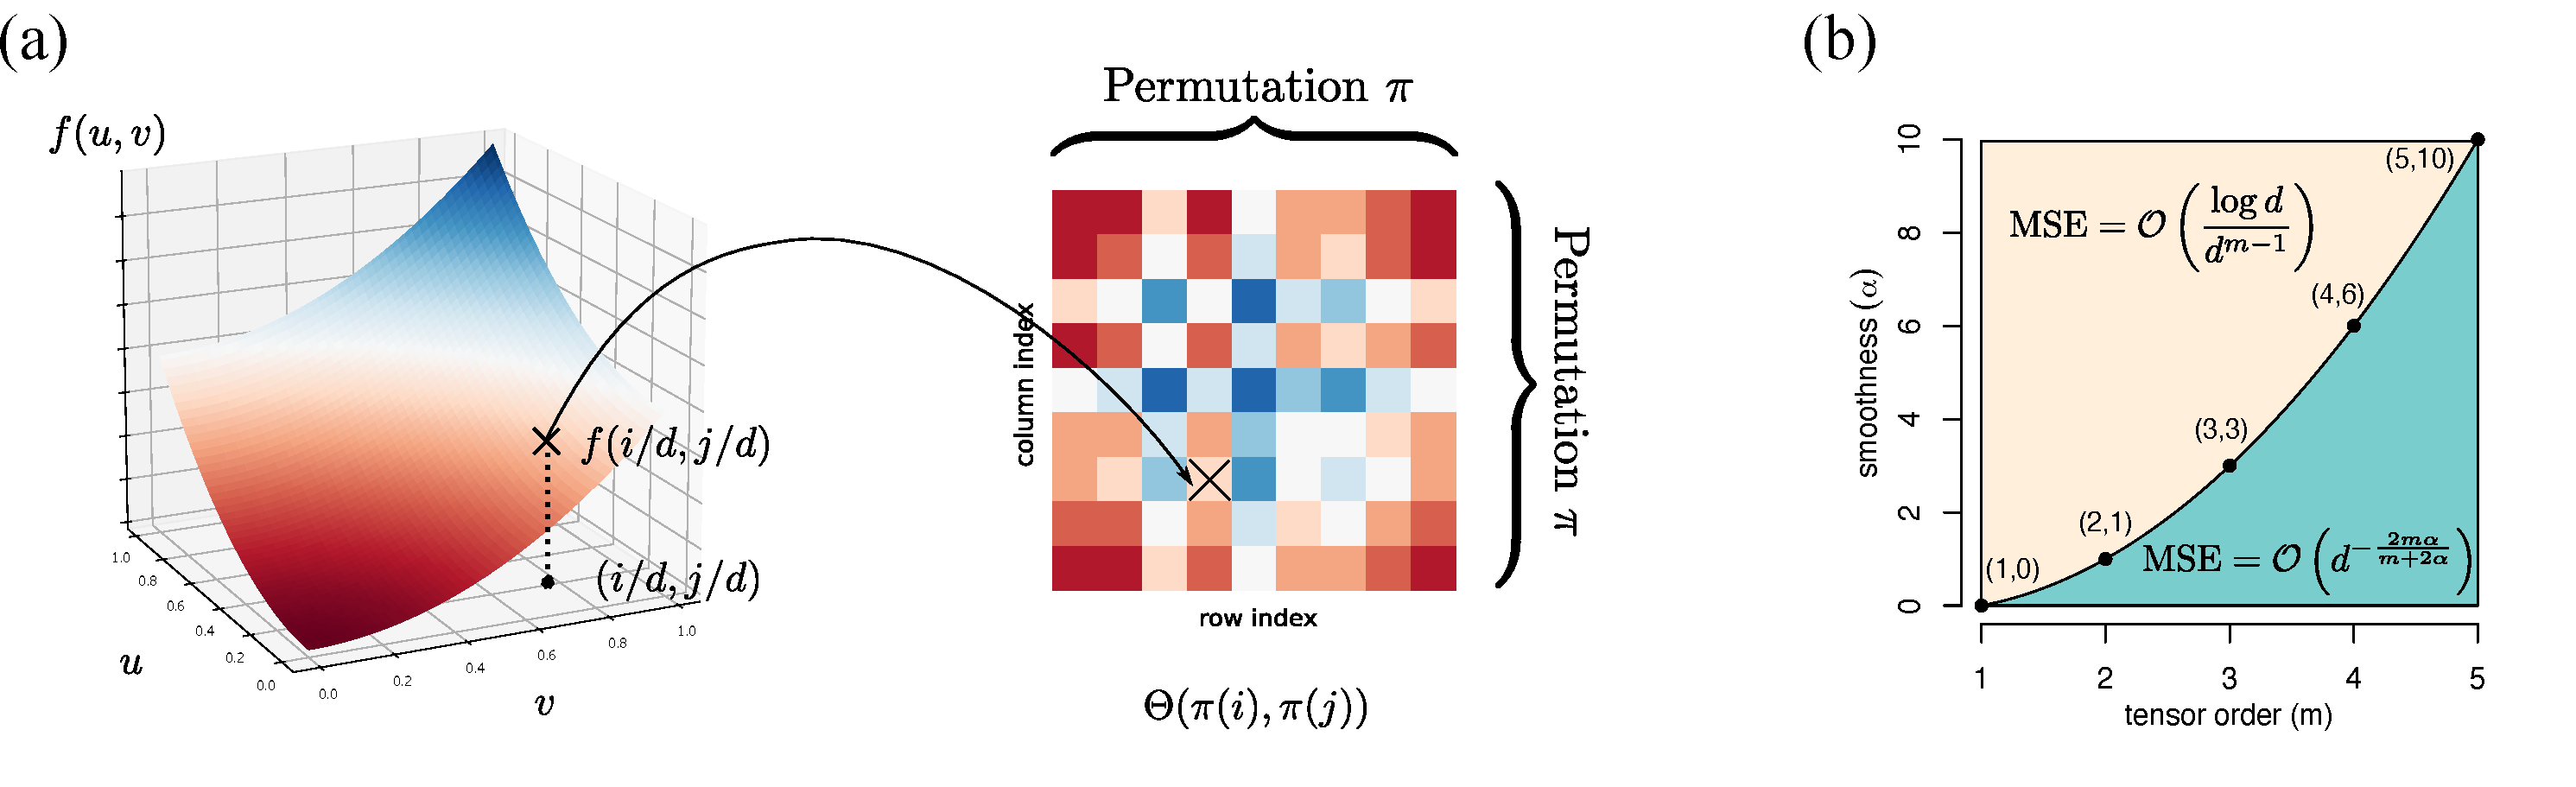
\includegraphics[width = .8\textwidth]{semantic.pdf}
    \caption{(a): Illustration of order-$m$ $d$-dimensional permuted smooth tensor models with $m=2$. (b): Regimes of mean square error (MSE) depending on the smoothness $\alpha$ and  tensor order $m$. Bold dots show the critical smoothness $\alpha^*$ and tensor order $m$. }
    \label{fig:rate}
   \vspace{-.5cm}
\end{figure}

Tensor estimation problem cannot be solved without imposing structure. 
% An appropriate reordering of tensor entries can provide effective representation of the hidden signal structure.
% We develop a \emph{permuted} smooth tensor model based on this motivation. %Our primary goal is to estimate a permuted smooth signal tensor from a noisy observation.%(formal definition of smoothness is deferred to Section~\ref{sec:md}). 
%For simplicity of notation; we focus on symmetric tensors in the main paper; our models and techniques easily generalize to non-symmetric tensors.
We study a class of structured tensors, \emph{permuted smooth tensors} of the following form:
%Let $\tY$ be an order-$m$ $d$-dimensional symmetric tensor generated from the model,
\begin{align}\label{eq:gmd}
    \tY = \Theta\circ \pi + \text{noise}, \quad \text{where}\quad \Theta_{i_1,\ldots,i_K}=f(i_1,\ldots,i_m),
\end{align}
where $\pi\colon[d]\rightarrow[d]$ is an unknown latent permutation, $\Theta$ is an unknown order-$m$ $d$-dimensional signal tensor, and $f$ is an unknown multivariate function with smoothness index $\alpha>0$; see Figure~\ref{fig:rate}(a) for an illustration. Our primary goal is to estimate a permuted smooth signal tensor from a noisy observation. 

{\bf Related work and our contributions.} The estimation problem of~\eqref{eq:gmd} falls into the general category of structured learning with \emph{latent permutation}, which has recently observed a surge of interest. Models involving latent permutations include graphon~\cite{chan2014consistent,gao2018minimax,klopp2017oracle}, stochastic transitivity models~\cite{chatterjee2015matrix,shah2019low}, statistical seriation~\cite{flammarion2019optimal,hutter2020estimation}, graph matching~\cite{ding2021efficient,livi2013graph}, and crowd labeling~\cite{shah2020permutation}. Most of theses methods are developed for matrices. The tensor counterparts, however, are far less well understood. Table~\ref{tab:comp} summarizes the related works on tensor learning with latent permutations. 

\begin{table*}[http]
    \centering
    \resizebox{\textwidth}{!}{%
    \begin{tabular}{c|cccc}
    & Pananjady et al~\cite{pananjady2020isotonic}&  Balasubramanian~\cite{balasubramanian2021nonparametric}&  Li et al~\cite{li2019nearest}&\textbf{Ours$^*$}\\
    \hline
       model structure& monotonic & Lipschitz & Lipschitz &  $\alpha$-smoothness  \\
     minimax lower bound& $\surd$  & $\times$ & $\times$ & $\surd$ \\
     error rate for order-3 tensors& $d^{-1}$ & $d^{-6/5}$ & $d^{-1}$ & $d^{-2}$ \\
     polynomial algorithm& $\surd$ &$\times$ & $\surd$ & $\surd$\\
        \hline
    \end{tabular}
    }
    \caption{\small Comparison of our results with previous works. $^*$We list here only the result for infinitely smooth order-3 tensors. Our results allow general tensors of arbitrary order $m$ and smoothness $\alpha$; See Theorems~\ref{thm:LSE} and \ref{thm:BC}.}\label{tab:comp}
\end{table*}

 
%Notice that the unknown permutation setting incurs identifiability issue. We cannot estimate both signal tensor and permutation. To avoid this identifiability issue, we measure the performance of the estimation by mean square error of the permuted signal tensor $\Theta\circ\pi$. 
%{\bf Contributions:}
The primary goal of our work is to provide statistical and computational estimation accuracy for the permuted smooth tensor model~\eqref{eq:gmd}.  
%and its statistical hardness in terms of minimax rate, and construct a polynomial-time algorithm for the estimation.
%We propose two estimating algorithms with accuracy guarantees: the least square estimation and Borda count estimation. 
We summarize our major contributions below. 
\begin{enumerate}[label={(\alph*)},wide,topsep=-3pt,itemsep=0pt,parsep=1pt]
\item We develop a general permuted $\alpha$-smooth tensor model for an arbitrary smoothness index $\alpha>0$. In contrast to earlier work~\cite{balasubramanian2021nonparametric,li2019nearest} that focuses only on $\alpha=1$, we fully establish the statistically optimal error rate and its dependence on tensor order, dimension, and smoothness index. 
%We establish the upper bound of the least-square estimate with high probability and show that this upper bound matches with minimax lower bound implying its optimality. 
\item We discover an intriguing phase transition phenomenon with respect to the smoothness threshold needed for optimal tensor recovery in model~\eqref{eq:gmd}. The critical threshold $\alpha^*$ (defined in Theorem~\ref{thm:LSE} and ~\ref{thm:BC}) characterizes two distinct error dependence behaviors on the smooth index $\alpha$. We proved that the error decreases with $\alpha$ in the range $\alpha<\alpha^*$, whereas the error is a constant of $\alpha$ in the range $\alpha>\alpha^*$. Figure~\ref{fig:rate}(b) plots the critical smoothness $\alpha^*$ as a function of tensor order $m$. 
%In addition, we prove that the optimal approximation degree of polynomial is $\min(\lceil \alpha\rceil, m(m-1)/2)$, where $\alpha$ is the smoothness of a tensor and $m$ is the order of a tensor. 
%The results implies that a polynomial of degree of $\alpha^*$ is sufficient for accurate recovery of order-$m$ tensors, whereas higher smoothness exhibits no further benefits.
These results are distinct from the matrix counterparts~\citep{gao2016optimal,klopp2017oracle,gao2018minimax}, thereby highlighting the fundamental challenges with tensors. 


\item We provide an efficient polynomial-time Borda count algorithm that provably achieves optimal rate under monotonicity assumptions. Simulation and data studies demonstrate the competitive performance of our algorithm.
\end{enumerate}


{\bf Notation.} We use $[d]=\{1,\ldots,d\}$ for $d$-set with $d\in\mathbb{N}_{+}$. For a set $S$, $|S|$ denotes its cardinality and $\mathds{1}_S$ denotes the indicator function. For positive two sequences $\{a_n\},\{b_n\}$,  we denote $a_n\lesssim b_n$ if $\lim_{n\to\infty} a_n/b_n\leq c$ for some constant $c>0$, and $a_n\asymp b_n$ if $c_1\leq \lim_{n\to \infty} a_n/b_n\leq c_2$ for some constants $c_1,c_2>0$. Given number $a\in\mathbb{R}$, the floor function $\lfloor a\rfloor$ is the largest integer no greater than $a$, and the ceiling function $\lceil a\rceil$ is the smallest integer no less than $a$.
We use $\tO(\cdot)$ to denote the big-O notation, $\tilde \tO(\cdot)$ the variant hiding logarithmic factors. An event $A$ is said to occur \emph{with high probability} if $\mathbb{P}(A)$ tends to 1 as the tensor dimension $d\to\infty$. Let $\Theta\in\mathbb{R}^{d\times \cdots \times d}$ be an order-$m$ $d$-dimensional tensor, and $\pi\colon[d]\rightarrow[d]$ be an index permutation. We use $\Theta_{i_1,\ldots,i_m}$ to denote the tensor entry indexed by $(i_1,\ldots,i_m)$, and use $\Theta\circ\pi$ to denote the permuted tensor such that $(\Theta\circ\pi)_{i_1,\ldots,i_m} = \Theta_{\pi(i_1),\ldots,\pi(i_m)}$ for all $(i_1,\ldots,i_m)\in[d]^m$. We use $S(d)=\{\pi\colon [d]\to[d]\}$ to denote all possible permutations on $[d]$.
\vspace{-.2cm}
\section{Smooth tensor model with unknown permutation}\label{sec:md}
\vspace{-.2cm}
Suppose we observe an order-$m$ $d$-dimensional symmetric data tensor from the following model,
\begin{equation}\label{eq:obs}
\tY=\Theta\circ \pi+\tE,
\end{equation}
where $\pi\colon[d]\rightarrow[d]$ is an unknown latent permutation,  $\Theta\in \mathbb{R}^{d\times \cdots\times d}$ is an unknown symmetric signal tensor under certain smoothness (to be specified in next paragraph), and $\tE$ is a symmetric noise tensor consisting of zero-mean, independent sub-Gaussian entries with variance bounded by $\sigma^2$. For simplicity of presentation, we focus on symmetric tensors in the main paper; our models and techniques easily generalize to non-symmetric tensors. Here, we do not assume identical distributions among entries in $\tE$. In particular, we allow the error variance to depend on mean. Therefore, our model~\eqref{eq:gmd} allows a wide range of data types including Gaussian and Bernoulli tensors. 

We now describe the smooth model on the signal $\Theta$. Assume that there exists a multivariate function $f\colon [0,1]^m\rightarrow \mathbb{R}$ underlying the signal tensor, such that
\begin{align}\label{eq:rep}
\Theta_{i_1,\ldots,i_m} = f\left({i_1\over d},\ldots,{i_m\over d}\right).
\end{align}
Assume the generating function $f$ is in the $\alpha$-H\"older smooth family. 
\begin{defn}[$\alpha$-H\"older smooth]
A function $f\colon [0,1]^m\rightarrow \mathbb{R}$ is $\alpha$-H\"older smooth, denoted as $f\in\tH(\alpha)$, if there exists a polynomial $P_{\lfloor \alpha\rfloor}(\mx-\mx_0)$ of degree  $\lfloor \alpha\rfloor$, such that 
\begin{align}\label{eq:defn}
    |f(\mx) - P_{\lfloor \alpha\rfloor}(\mx-\mx_0)| \leq C\|\mx-\mx_0\|_\infty^\alpha,
\end{align}
for all $\mx,\mx_0\in [0,1]^m$ and a universal constant $C>0.$
\end{defn}
H\"older smooth function class is one of the most popular function classes considered in the nonparametric regression literature \citep{klopp2017oracle,gao2018minimax}. In addition to the function class $\tH(\alpha)$, we also define the smooth tensor class based on discretization~\eqref{eq:rep}, 
\[
{\small \tP(\alpha)= \left\{\Theta\in\mathbb{R}^{d\times \cdots \times d} \colon\Theta(\omega) = f\left({\omega \over d}\right) \text{ for all } \omega=(i_1,\ldots,i_m) \in[d]^m \text{ and } f\in\tH(\alpha)\right\}.}
\]
Combining~\eqref{eq:obs} and~\eqref{eq:rep} yields our proposed \emph{permuted smooth tensor model}. The generating process is visualized in Figure~\ref{fig:rate}(a) for the case $m=2$ (matrices). 

We give two concrete examples to show the applicability of our permuted smooth tensor model. 

\begin{example}[Four-player game tensor] Consider a four-player board game. Suppose there are in total $d$ players, among which all combinations of four have played against each other. The game results are naturally summarized as an order-4 (asymmetric) tensor, with entries encoding the winner of four-player games. Our model is then given by
\begin{align}
\mathbb{E}(Y_{i_1,\ldots,i_4})&=\mathbb{P}(\text{user $i_1$ wins over $(i_2,i_3,i_4)$})
=f\left({\pi(i_1)\over d},\cdots, {\pi(i_4)\over d}\right).
\end{align}
In this setting, we can interpret the permutation $\pi$ as the unknown ranking among $d$ players, and the function $f$ the unknown four-players interaction. Operationally, players with similar ranking would have similar performance encoded by the smoothness of $f$. 
\end{example}

\begin{example}[Co-authorship networks] Consider co-authorship networks. Suppose there are in total $d$ authors. We say there exists a hyperedge between nodes $(i_1,\ldots,i_m)$ if the authors $i_1,\ldots,i_m$ have co-authored at least one paper. The resulting hypergraph is represented as an order-$m$ (symmetric) adjacency tensor. Our model is then expressed as
\begin{align}
    \mathbb{E}(Y_{i_1,\ldots,i_m})&=\mathbb{P}(\text{authors $i_1,\ldots,i_m$ co-authored})
=f\left({\pi(i_1)\over d},\cdots, {\pi(i_m)\over d}\right).
\end{align}
In this setting, we can interpret the permutation $\pi$ as the affinity measures of authors, and the function $f$ represents the $m$-way interaction among authors.
%check examples from~\cite{ke2019community}. 
\end{example}



% \subsection{Connection to previous work}\label{sec:priorwork}
% The signal model~\eqref{eq:rep} has close relation to two different problems: multivariate nonparametric regression and hypergraphon estimation. 

% First,  one may view the problem as the classical nonparametric regression problem modeling the mean $(\Theta\circ\pi)_{i_1,\ldots,i_m}$ from  a regression function $f$ with covariates $({i_1}/d,\ldots,{i_m}/d)$. However, in our setting, we cannot observed the permutation $\pi$, which makes the problem  more difficult. Unlike the classical nonparametric regression, the function $f$ should be estimated only from  the observed noisy tensor $\{\tY_{i_1,\ldots,i_m}\}$ without information of the permutation. 
% In addition, this unobserved permutation setting incurs identifiability issue. We cannot estimate both the function $f$ (equivalently $\Theta$) and the permutation $\pi$. To overcome this identifiability issue, we use the following mean squared error for the permuted signal tensor $\Theta\circ\pi$ to measure the performance of the estimation,
% \begin{align}
%     \frac{1}{d^m}\sum_{(i_1,\ldots,i_m)\in[d]^m}\left((\hat\Theta\circ\hat\pi)_{i_1,\ldots,i_m}-(\Theta\circ\pi)_{i_1,\ldots,i_m}\right)^2.
% \end{align}
% Leveraging the underlying structure in \eqref{eq:rep} and smoothness of the function $f$ (formal definition is deferred to Section~\ref{subsec:bm}), we overcome these difficulties and successfully estimate the signal tensor without observing the permutation.

% In addition, the model~\eqref{eq:rep} is related to hypergraphons. 
% A  hypergraph is a generalization of a graph in which an edge (called hyperedge) can join any number of vertices.  $m$-uniform hypergraph is a hypergraph of which all hyperedges have size $m$. The structure of $m$-uniform hypergraph is naturally represented by a $m$-order tensor. So one can view the problem \eqref{eq:gmd} as estimating the probability tensor generating the observed hypergraph.
% The theory of hypergraph limits has studied and introduce hypergraphons  \citep{gowers2007hypergraph,zhao2015hypergraph} similar to graphons, limits of a sequence of graph \citep{lovasz2006limits,diaconis2007graph,lovasz2012large}.    Unlike the matrix case where graphon is represented as a bivariate function~\citep{lovasz2012large}, however, hypergraphons for $m$-uniform hypergraphs should be represented as a $(2^m-2)$-variate function \citep{zhao2015hypergraph}. Due to exponential number of variates, the general hypergraphon suffers from  high sample complexity. 
% To overcome this issue, simple $m$-variate hypergraphons have been introduced recently for efficient estimation while trading off the model flexibility \citep{balasubramanian2021nonparametric,lyu2021latent}.
%  Although our model can be viewed as a simple $m$-variate hypergraphon, our main interests lie on the general estimation of the smooth signal tensor from noisy observation including both binary- and continuous-valued entries.
\vspace{-.2cm}
\section{Block-wise tensor approximation }\label{sec:tba}
\vspace{-.2cm}
Our general strategy for estimating the signal tensor is based on the block-wise tensor approximation. We first introduce the tensor block model~\citep{wang2019multiway,han2020exact}. Then, we extend this model to the block-wise polynomial approximation.
\vspace{-.2cm}
\subsection{Tensor block model}
\vspace{-.2cm}
The tensor block model describes a checkerbroad pattern in the signal tensor. Specifically, suppose that there are $k$ clusters in the tensor dimension $d$, and the clusters are represented by a clustering function $z\colon [d]\rightarrow  [k]$. Then, the tensor block model assumes that signal tensor $\Theta\in\mathbb{R}^{d\times \cdots \times d}$ takes values from a mean tensor $\tS\in\mathbb{R}^{k\times\cdots\times k}$ according to the clustering function $z$:
\begin{align}\label{eq:block}
    \Theta_{i_1,\ldots,i_m} = \tS_{z(i_1),\ldots,z(i_m)}, \quad \text{ for all } (i_1,\ldots,i_m)\in[d]^m.
\end{align}
A tensor $\Theta$ satisfying~\eqref{eq:block} is called a block-$k$ tensor. The tensor block model has shown great success in discovering hidden group structure in many applications including hypergraph clustering \citep{ke2019community}, collaborative filtering \citep{zhang2021dynamic} and signal dehe ection in 3D/4D
imaging \citep{zhang2020denoising}.
Despite its popularity and great applicability, the tensor block models cannot describe delicate structure of the signal tensor when the tensor dimension $d$ is very large. 
% \fixme{Miaoyan}{two common pitfalls I have pointed before. 1) ``it is'' is a weak subject. 2) ``not reasonable'' should be replaced by a single word. I did not change these two on purpose, in order to draw your attention. Please correct them (and others in the entire paper). }\fixme{Chanwoo}{That makes sense! thank you}
% \fixme{Miaoyan}{alternatively, use/mix the following sentence.}
This parametric model aims to explain data with a finite number of blocks; this approach is useful when the sample outsizes the parameters. Our nonparametric models~\eqref{eq:rep}, on the other hand, use infinite number of parameters to allow growing model complexity as sample increases. 
Therefore, we shift the goal of tensor block model from discovering hidden group structure to approximating the generative process of the function $f$ in~\eqref{eq:rep}. Thus, the number of blocks $k$ should be interpreted as a resolution parameter (i.e., a bandwidth) of the approximation similar to the notion of number of bins in histogram and polynomial regression. 
\vspace{-.2cm}
\subsection{Block-wise polynomial approximation}\label{sec:poly}
\vspace{-.2cm}
The tensor block model~\eqref{eq:block} can be viewed as a discrete version of piece-wise \emph{constant} function with $\alpha=0$ in~\eqref{eq:defn}. This connection motivates us to use block-wise \emph{polynomial} tensors to approximate $\alpha$-H\"older functions. Now we extend~\eqref{eq:block} to block-wise polynomial models. For a given block number $k$, we use $z\colon[d]\rightarrow [k]$ to denote the canonical clustering function that partitions $[d]$ into $k$ clusters,
\begin{align}
    z(i) = \lceil ki/d\rceil, \quad \text{ for all } i\in[d].
\end{align}
The collection of inverse images $\{z^{-1}(j)\colon j\in[k]\}$ consists of  disjoint and equal-sized subsets in $[d]$, and we have $\cup_{j\in[k]}z^{-1}(j) = [d]$ by the construction. We denote $\tE_k$ as the $m$-way partition as a collection of $k^m$ disjoint, equal-sized blocks in $[d]^m$, such that 
\begin{align}\label{eq:blockind}
    \tE_k = \{z^{-1}(j_1)\times\cdots\times z^{-1}(j_m)\colon (j_1,\ldots,j_m)\in [k]^m\}.
\end{align}
We propose to approximate the signal tensor $\Theta$ in~\eqref{eq:rep} by degree-$\ell$ polynomial tensor within each $\tE_k$-block. Specifically, we use $\caliB(k,\ell)$ to denote the class of block-$k$, degree-$\ell$ polynomial tensors,
\begin{align}
    \caliB(k,\ell) = \bigg\{&\tB\in(\mathbb{R}^d)^{\otimes m}\colon \tB(\omega) = \sum_{\Delta\in\tE_k}\text{Poly}_{\ell,\Delta}(\omega)\mathds{1}\{\omega\in\Delta\}\text{ for all } \omega\in[d]^m\bigg\},
\end{align}
where $\text{Poly}_{\ell,\Delta}(\cdot)$ denotes a degree-$\ell$ polynomial function in $\mathbb{R}^m$. Notice that degree-0 polynomial block tensor reduces to the tensor block model \eqref{eq:block}. We genealized the tensor block model to degree-$\ell$ polynomial block tensor, in a way that is analogous to the generalization from $k$-bin histogram to $k$-piece-wise polynomial regression in nonparametric statistics~\cite{wasserman2006all}.

Smoothness of the function $f$ in \eqref{eq:rep} turns out to play an important role in the block-wise polynomial approximation.
% We define the class of $\alpha$-H\"older smooth functions $\tH(\alpha)$.
% \begin{defn}[$\alpha$-H\"older smooth]
% A function $f\colon [0,1]^m\rightarrow \mathbb{R}$ is $\alpha$-H\"older smooth denoted as $f\in\tH(\alpha)$ if there exists a polynomial $P_{\lfloor \alpha\rfloor}(\cdot-\mx_0)$ of degree  $\lfloor \alpha\rfloor$, such that 
% \begin{align}
%     |f(\mx) - P_{\lfloor \alpha\rfloor}(\mx-\mx_0)| \leq C\|\mx-\mx_0\|_\infty^\alpha,
% \end{align}
% for all $\mx,\mx_0\in [0,1]^m$ and universal constant $C>0.$
% \end{defn}
The following lemma explains the role of smoothness in the approximation. 
\begin{lem}[Tensor block approximation]\label{lem:approx}
Suppose  $\Theta\in\tP(\alpha)$. Then,
for every block number $k\leq d$, and degree $\ell\in\{0\}\cup\mathcal{N}_+$, we have the approximation error
\begin{align}
   \inf_{\tB\in\caliB(k,\ell)} \frac{1}{d^m}\FnormSize{}{\Theta-\tB}^2\lesssim \frac{m^2}{k^{2\min(\alpha,\ell+1)}}.
\end{align}
\end{lem}
This theorem implies that we can always find block-wise polynomial tensor close to the signal tensor generated from $\alpha$-H\"older smooth function $f$.


\vspace{-.2cm}
\section{Fundamental limits via least-squares estimation}\label{sec:lse}
\vspace{-.2cm}
We propose two estimation methods based on the block-wise polynomial approximation. We first introduce a statistically optimal but computationally infeasbile least-squares estimator. The least-squares estimation serves as statistical benchmark because it achieves the minimax lower bound. In Section~\ref{sec:borda}, we will present a polynomial-time algorithm with provably same optimal rates under monotonicity assumptions.

We propose the least-squares estimator for the signal tensor and the permutation $(\Theta,\pi)$ by minimizing the Frobenius loss under block-$k$, degree-$\ell$ polynomial tensor family $\caliB(k,\ell)$, 
\begin{align}\label{eq:lseopt}
    (\hat\Theta^{\text{LSE}},\hat \pi^{\text{LSE}}) &= \argmin_{\Theta\in\caliB(k,\ell), \  \pi\in S(d)}\FnormSize{}{\tY-\Theta\circ\pi}.
\end{align}
The least-squares estimator $(\hat\Theta^{\text{LSE}},\hat\pi^{\text{LSE}})$ depends on two tuning parameters: the number of blocks $k$ and the polynomial degree $\ell$. The optimal choice $(k^*,\ell^*)$ is provided in our next theorem. The result establishes the upper bound for the mean squared error of the least square estimator~\eqref{eq:lseopt}. 
\begin{thm}[Least-squares estimation error]\label{thm:LSE} 
Consider the order-$m$ ($m\geq 2$) permuted smooth tensor model~\eqref{eq:obs} with $\Theta\in\tP(\alpha)$.
Let $(\hat\Theta^{\textup{LSE}},\hat\pi^{\textup{LSE}})$ denote the least-squares estimates with a given $(k,\ell)$ in \eqref{eq:lseopt}. Then, the estimator $\hat\Theta^{\textup{LSE}}\circ\hat\pi^{\textup{LSE}}$ satisfies 
\begin{align}\label{eq:rateMSE}
    \frac{1}{d^m}&\FnormSize{}{\hat\Theta^{\textup{LSE}}\circ\hat\pi^{\textup{LSE}}-\Theta\circ \pi}^2\lesssim  \frac{m^2}{k^{2\min(\alpha,\ell+1)}}+ \frac{k^m(\ell+m)^\ell}{d^m}+\frac{\log d}{d^{m-1}},
\end{align}
with very high probability.
In particular, setting $\ell^* = \min(\lceil\alpha\rceil,m(m-1)/2)-1 $ and $k^* = \lceil d^{m\over m+2\min(\alpha,\ell^*+1)}\rceil$ yields the bound as 
\begin{align}\label{eq:rates}
     \eqref{eq:rateMSE}\lesssim \begin{cases}d^{-{2m\alpha\over m+2\alpha}} & \text{ when } \alpha < \frac{m(m-1)}{2},\\{\log d\over d^{m-1}}&\text{ when } \alpha \geq \frac{m(m-1)}{2}.\end{cases}
\end{align}
\end{thm}
We discuss the asymptotic error rates as $d\rightarrow \infty$ while treating the tensor order $m$ and smoothness $\alpha$ fixed. 
The least square estimation error has two sources of error: the nonparametric error $d^{-{2m\alpha\over m+2\alpha}}$ and the clustering error $\log d/d^{m-1}$.  When the function $f$ is smooth enough, estimating the function $f$ becomes relatively easier compared to estimating the permutation $\pi$. This intuition coincides with the fact that the clustering error dominates the nonparametric error when  $\alpha\geq m(m-1)/2$. 


%\begin{figure}[h]
%    \centering
%    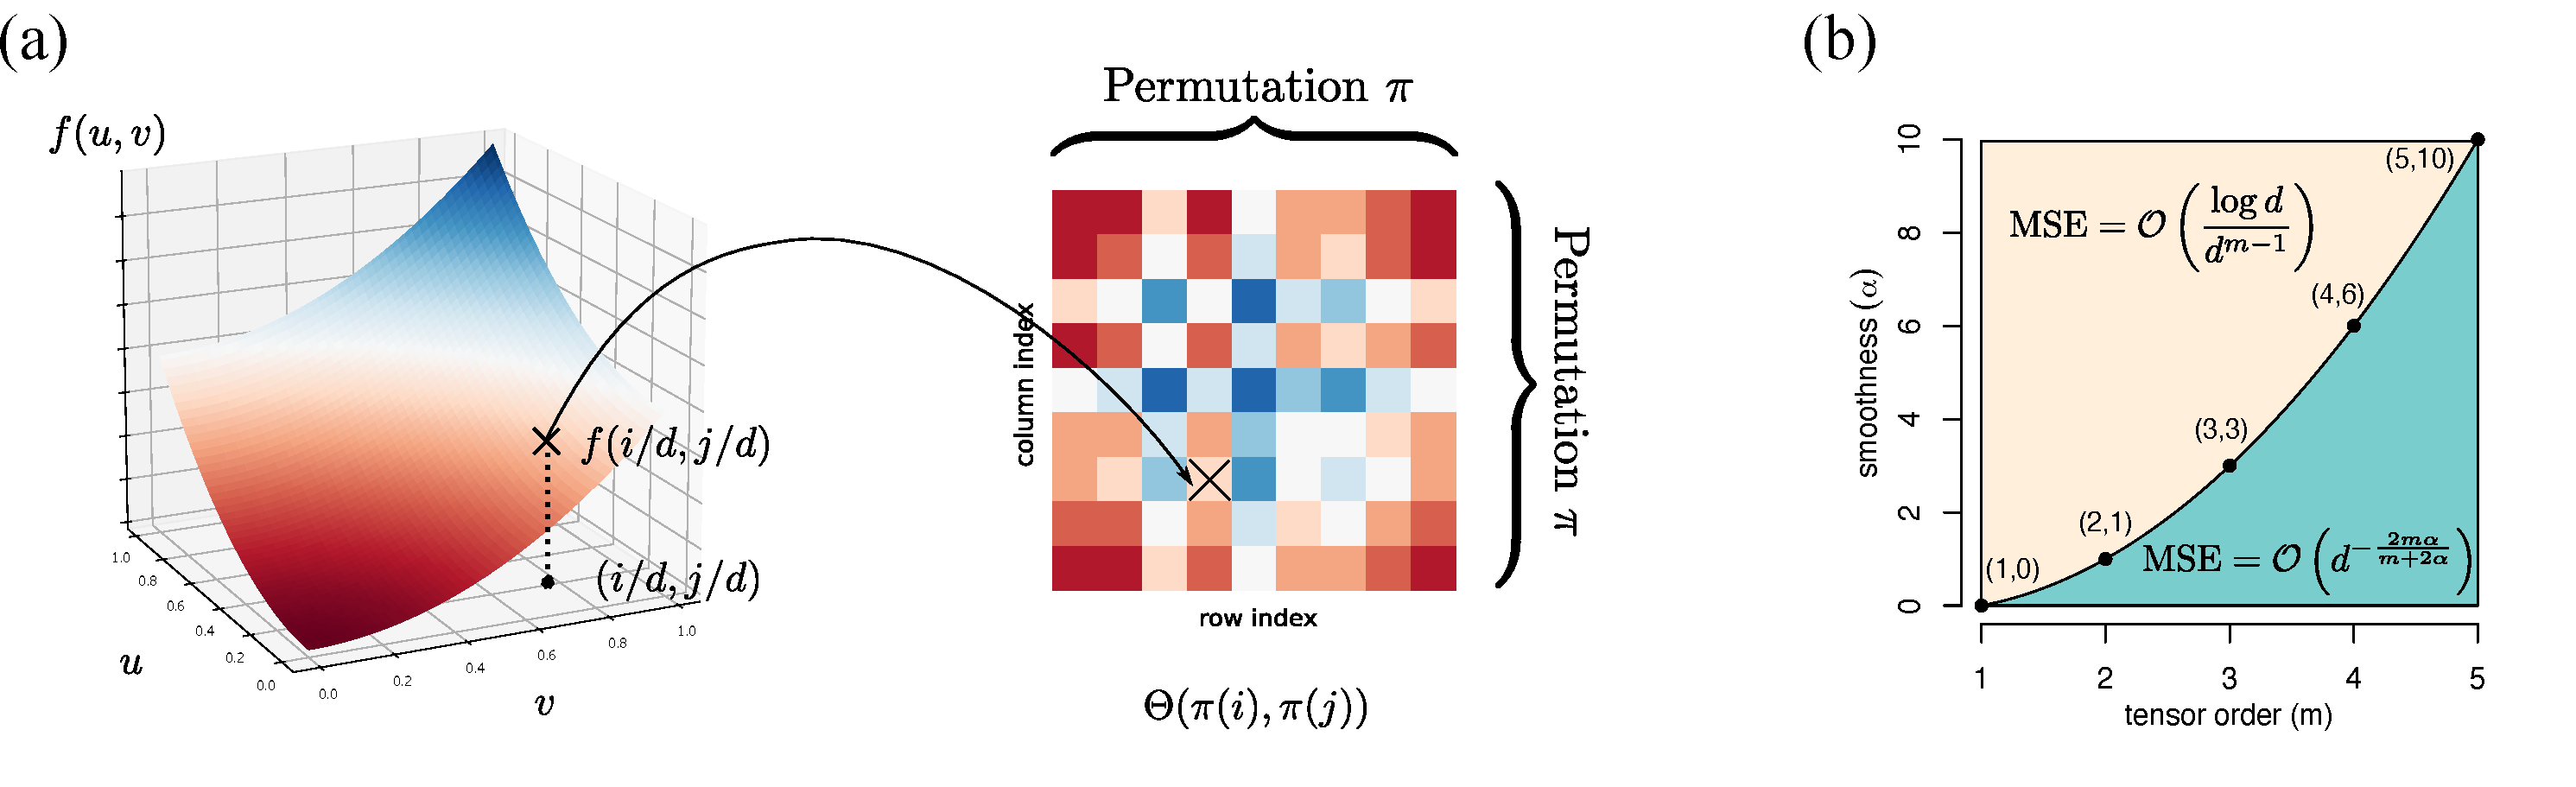
\includegraphics[width = .8\textwidth]{semantic.pdf}
%    \caption{(a): Realization of signal tensor from generating function $f$ where $(u_i,u_j) = (i/d,j/d)$. The figure is modified from \cite{airoldi2013stochastic}. (b): Mean square error rate of the least square estimator with respect to tensor dimension $d$. }
  %  \label{fig:rate}
 %   \vspace{-.5cm}
%\end{figure}




We now compare our results with existing work in the literature. Based on Theorem~\ref{thm:LSE}, the best rate is obtained with the choice of  $(\ell^*, k^*) = (0,\lceil d^{1\over\alpha\wedge1+1}\rceil)$ in the matrix case ($m =2$). This block-wise constant approximation and convergence rate reduce to the results in  \cite{gao2016optimal,klopp2017oracle}. Therefore, the least square estimation achieves the minimax optimal rate in matrix case. Furthermore, we solve the conjectured optimal convergence rate in \cite{balasubramanian2021nonparametric} for higher order tensor case ($m\geq 3$). This improvement stems from polynomial tensor approximation in Lemma~\ref{lem:approx}. The work in
\cite{balasubramanian2021nonparametric} considers only the block-wise constant approximation  ($\ell = 0$). This restriction results in sub-optimality because the optimal degree $\ell^*$ is shown to be greater than 0 for higher-order tensors. For example, order-3 $\alpha$-smooth tensors have the optimal degree and block size as $(\ell^*,k^*) = (2,\lceil d^{1/3}\rceil)$ for all $\alpha\geq 2.$  This result shows the clear difference from matrices and highlights the challenges with  tensors. 

We now show that the upper bound of Theorem~\ref{thm:LSE} is not only minimax optimal for the matrices but also for higher-order tensors.
The result is based on information-theoretical analysis that combines the minimax rate for nonparametric and permutation estimation. Our minimax lower bound applies to all estimators including, but not limited to, least square estimator and all polynomial-time estimators. 
\begin{thm}[Minimax lower bound]\label{thm:minimax}For any given $\alpha\in(0,\infty)$, the estimation problem based on model~\eqref{eq:gmd} obeys the minimax lower bound 
\begin{equation}\label{eq:minimax}
\inf_{(\hat \Theta,\hat \pi)}\sup_{\Theta\in \tP(\alpha), \pi\in S(d)} \mathbb{P}\left({1\over d^m}\FnormSize{}{\Theta\circ \pi-\hat \Theta\circ \hat \pi}^2 \gtrsim d^{-{2m\alpha\over m+2\alpha}}+d^{-(m-1)}\log d \right) \geq 0.8.
\end{equation}
\end{thm}
We see that the lower bound matches the upper bound in Theorems~\ref{thm:LSE}. Therefore,
the least square estimator \eqref{eq:lseopt}  is statistically optimal.


% There are two ingredients in the rate of convergence, the nonparametric rate $ d^{-2m(\alpha\wedge 1)\over m+2(\alpha\wedge 1)}$ and the clustering rate $\log d/d^{m-1}$.
% Depending on constants tensor order $m$ and smoothness $\alpha$, the convergence rate in \eqref{eq:rateMSE} becomes 
% \begin{align}
%      d^{-2m(\alpha\wedge1)\over m+2(\alpha\wedge1)}+\frac{\log d}{d^{m-1}}\asymp \begin{cases} d^{-2\alpha\over 1+\alpha}& m = 2, \alpha\in(0,1),\\ \log d/d & m =2, \alpha = 1,\\ d^{-2m(\alpha\wedge 1)\over m+2(\alpha\wedge 1)} & m>2.\end{cases}
% \end{align}
% Notice that the nonparametric rate dominates the clustering rate when $m>2$. The intuitive  explanation for this phenomenon is that when tensor order $m$ increases, the nonparametric estimation becomes harder because the number of parameters increases exponentially due to the possible $m$-combinations from $k$ clusters. On the other hand, the difficulty of clustering problem are almost the same regardless of tensor order $m$. This is because the number of clusters $k$ and tensor dimension $d$ remain the same.


\vspace{-.2cm}
\section{An adaptive and computationally feasible procedure}\label{sec:borda}
\vspace{-.2cm}
At this point, we should point out that computing the least square optimizer $(\hat\Theta^{\text{LSE}},\hat\pi^{\text{LSE}})$ in \eqref{eq:lseopt} with polynomial-time algorithm is unknown. We suspect that the algorithm for \eqref{eq:lseopt} may be computationally intractable. In this section, we propose an efficient polynomial-time \emph{Borda count} algorithm. Furthermore, we show that Borda count estimator actually achieves the same convergence rate as the minimax lower bound under the $\beta$-monotonicity condition. 
\vspace{-.2cm}
\subsection{Borda count algorithm}
\vspace{-.2cm}
We first introduce $\beta$-monotonicity for the generating functions.  
\begin{defn}[$\beta$-monotonicity]\label{eq:defn}
A function $f\colon[0,1]^m \rightarrow \mathbb{R}$ is called $\beta$-monotonic, denoted as $f\in\tM(\beta)$, if 
\begin{align}\label{eq:monotonic}
    \left({i-j\over d}\right)^{1/\beta}\leq g(i)-g(j),\quad \text{ for all } i>j\in[d],
\end{align}
where we define $g(i) = d^{-(m-1)}\sum_{(i_2,\ldots,i_m)\in[d]^m} f\left({i\over d},{i_2\over d},\ldots,{i_m\over d}\right)$ for all $i \in[d].$
\end{defn}

This $\beta$-monotonicity condition can be viewed as an extension of the strict monotonic degree condition in binary-valued networks~\citep{chan2014consistent} to general setting. Consider the hypergraph example where the observed tensor $\tY$ is the adjacency tensor representing the connectivity among $d$-nodes. Then, the function $g$ is the degree function of the nodes. Our $\beta$-monotonicity condition is also closely related to isotonic functions~\citep{han2019isotonic,pananjady2020isotonic} which assume the coordinate-wise monotonicity, i.e., $f(x_1,\ldots,x_d)\leq f(x_1',\ldots,x_d')$
when $x_i\leq x_i'$ for $i\in[d]$. %The isotonic functions belong to the strict monotonic function class.

This $\beta$-monotonicity condition allows us to estimate the permutation $\pi$  in polynomial-time complexity. Before presenting the theoretical guarantees, we provide the intuition here. The parameter $\beta$ measures the difficulty of the problem for estimating the permutation $\pi$. Consider the noisy observation $\tY$ in  \eqref{eq:gmd}.
We define the scores function $\tau\colon [d]\rightarrow\mathbb{R}$ as
\begin{align}\label{eq:score}
    \tau(i) = \frac{1}{d^{m-1}}\sum_{(i_2,\ldots,i_m)\in[d]^m} \tY_{i,i_2,\ldots,i_m}.
\end{align}
Then, the permuted score function $\tau\circ\pi^{-1}$ is equivalent to the function $g$ in \eqref{eq:monotonic} for the noiseless case.
Therefore, we can find an estimate $\hat\pi$ that makes the permuted score function $\tau\circ\hat\pi^{-1}$ monotonically increasing. Notice that the estimated permutation $\hat\pi$ could be different from the oracle permutation $\pi$ due to the noise. We find that the larger $\beta$ guarantees the sharper consistency of $\hat\pi$. The large $\beta$ implies the large gaps of $|g(i)-g(j)|$ for $i\neq j\in[d]$. Therefore, we obtain similar ordering of $\{\tau(i)\}_{i=1}^d$ before and after the addition of the noise. This intuition is well represented by the following lemma.
\begin{lem}[Permutation error]\label{lem:permute}
Let $\hat\pi$ be the permutation that makes the permuted score function $\tau\circ \hat\pi^{-1}$  monotonically increasing. Then, we have
\begin{align}
   \textup{Loss}(\pi,\hat\pi):= \frac{1}{d}\max_{i\in[d]}|\pi(i)-\hat\pi(i)|\lesssim \left(\sigma d^{-(m-1)/2}\sqrt{\log d}\right)^{\beta},
\end{align}
with high probability.
\end{lem}


Now we introduce a Borda count estimator that consists of two stages. The full estimation procedure is illustrated in Figure~\ref{fig:borda}.

  {\bf Sorting stage}: The purpose of the sorting is to rearrange the observed tensor $\tY$ so that the score function $\tau$ of sorted tensor  is  monotonically increasing. We define a permutation $\hat\pi^{\text{BC}}$  such that
    \begin{align}\label{eq:permute}
        \tau((\hat\pi^{\text{BC}})^{-1}(1))\leq \cdots \leq \tau((\hat\pi^{\text{BC}})^{-1}(d)).
    \end{align}
    Then, we obtain a sorted observation $\tilde\tY$,
    \begin{align}
        \tilde\tY_{i_1,\ldots,i_m} = \tY_{(\hat\pi^{\text{BC}})^{-1}(i_1),\ldots,(\hat\pi^{\text{BC}})^{-1}(i_m)},
    \end{align}
for all $(i_1,\ldots,i_m)\in[d]^m.$ An example of sorted observation is shown in Figure~\ref{fig:borda}.

 {\bf Block-wise polynomial approximation stage}: Given degree $\ell$, we estimate the degree-$\ell$ polynomial block tensor based on the sorted observation $\tilde\tY$ solving the following optimization problem,
    \begin{align}\label{eq:bclse}
        \hat\Theta^{\text{BC}} = \argmin_{\tB\in\caliB(k,\ell)}\FnormSize{}{\tilde\tY-\Theta}.
    \end{align}
    The estimate $\hat\Theta^{\text{BC}}$  depends on two tuning parameters: the number of blocks $k$ and polynomial degree $\ell$. The optimal choice of $(k^*,\ell^*)$ is provided in Theorem~\ref{thm:BC}.
    Notice that the least square estimation in \eqref{eq:lseopt} requires combinatoric search for the permutation resulting in exponential time complexity. However, \eqref{eq:bclse} only requires to estimate the degree-$\ell$ polynomial block tensor. Therefore, this step easily reduces to a degree-$\ell$ polynomial regression problem within each block $\tE_k$. 
\begin{figure}[htp]
    \centering
    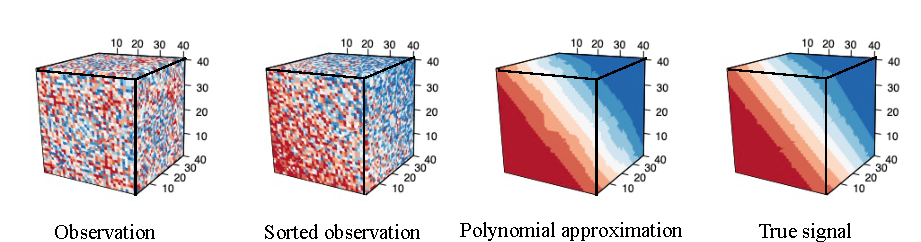
\includegraphics[width = .8\textwidth]{Borda.pdf}
    \caption{Procedure of Borda count estimation. We first sort the tensor entries using the proposed procedure. Then, we estimate the signal tensor using block-$k$ degree-$\ell$ polynomial approximation.}
    \label{fig:borda}
    \vspace{-.4cm}
\end{figure}
\vspace{-.2cm}
\subsection{Computational and statistical complexity}
\vspace{-.2cm}
%\paragraph{Complexity of the algorithm.}
The complexity of the Borda count algorithm can be computed separately in each stage.
In the sorting stage, computing the score function $\tau$  requires $\tO(d^{m-1})$ additions while sorting the $\tau(1),\ldots,\tau(d)$ takes about $\tO(d\log d)$ comparisons. In block-wise polynomial approximation stage, we compute $k^m$ different  degree-$\ell$ polynomial tensors. For each  degree-$\ell$ polynomial tensor,  $\tO((d/k)^m\ell)$ arithmetic operations are needed. Thus, the second step requires $\tO(d^m\ell)$ arithmetic operations.  Combining these two steps yields the total complexity at most $\tO(d^m\log d)$.

%\paragraph{Consistency of Borda count estimation.}
We show the consistency of the signal tensor estimation
based on  Lemma~\ref{lem:approx}-\ref{lem:permute}.
\begin{thm}[Estimation error for Borda count]\label{thm:BC}
Suppose that the signal tensor $\Theta$ is generated as in  \eqref{eq:rep} with $f\in\tH(\alpha)\cap \tM(\beta).$
Let $(\hat\Theta^{\textup{BC}},\hat\pi^{\textup{BC}})$ be the Borda count estimator in \eqref{eq:permute}-\eqref{eq:bclse} with a given $(k,\ell)$. Then, for every $k\leq d$ and degree $\ell\in \mathbb{N}_{\geq 0}$, we have
\begin{align}\label{eq:BC}
     \textup{MSE}(\hat\Theta^{\textup{BC}}\circ\hat\pi^{\textup{BC}},\ \Theta\circ\pi)\lesssim  \frac{m^2}{k^{2\min(\alpha,\ell+1)}}+ \frac{k^m(\ell+m)^\ell}{d^m}+ \left({\log d\over d^{m-1}}\right)^{\beta\min(\alpha,1)},
\end{align}
with high probability.
% with probability  $1-\exp\left(-C_2\left(d\log d +d^{m^2\over m+2(\alpha\wedge 1)}\right)\right)$.
\end{thm}
The three terms in the estimation bound~\eqref{eq:BC} correspond to approximation error (Lemma~\ref{lem:approx}), nonparametric error (Theorem~\ref{thm:LSE}), and permutation error (Lemma~\ref{lem:permute}), respectively. 
We find that the Borda count estimator achieves the same minimax-optimal rate as the least-squares estimator for sufficiently smooth tensors under Lipschitz score condition $\beta =1$. The least-squares estimator requires a combinatoric search with exponential-time complexity. By contrast, the Borda count estimator is polynomial-time solvable. Therefore, Borda count algorithm enjoys both statistical accuracy and computational efficiency. 


\vspace{-.2cm}
\section{Numerical comparisons}\label{sec:sim}
\vspace{-.2cm}
We simulate symmetric order-3 $d$-dimensional tensors based on the permuted smooth tensor model~\eqref{eq:rep} with function $f$ in Table~\ref{tb:md}. Notice that considered functions cover a reasonable range of model complexities from low rank to high rank. We generate the entries of the noise tensor i.i.d. from Gaussian distribution $N(0,0.5^2)$. The permutation $\pi$ is randomly sampled from all permutations from $[d]$ to $[d]$. 
Throughout all experiments, we evaluate the accuracy of the estimation by mean square error (MSE) $= d^{-3}\FnormSize{}{\Theta\circ\pi-\hat\Theta\circ\hat\pi}^2$ across $n_{\text{sim}} = 20$ replications.

 \begin{table}[htp]
     \vspace{-.2cm}
    \centering
    \caption{Smooth functions in simulation. We define the numerical CP/Tucker rank as the minimal rank $r$ for which the relative approximation error is below $10^{-4}$. The reported rank in the table is estimated from a $100\times100\times100$  signal tensor generated by \eqref{eq:rep}.\\ }
    \begin{tabular}{c|c|c|c}
        Model ID  &  $f(x,y,z)$ & CP rank & Tucker rank \\\hline
        1 &    $xyz$ & 1 & $(1,1,1)$\\
        2 & $(1+\exp(-3x^2+3y^2+3z^2))^{-1}$ &9& $(4,4,4)$ \\
        3 &  $\exp\left(-\max(x,y,z)-\sqrt{x}-\sqrt{y}-\sqrt{z}\right)$ &$\geq 100$& $(90,90,90$)
    \end{tabular}
    \vspace{-.2cm}
    \label{tb:md}
\end{table}

The first experiment examines the impact of the block number $k$ and degree of polynomial $\ell$ for the approximation. We fix the tensor dimension $d = 100$, and vary the number of blocks $k\in\{1,\ldots,15\}$ and polynomial degree $\ell\in\{0,1,2,3\}.$
Figure~\ref{fig:degk} demonstrates the trade-off in accuracy determined by the number of groups for each polynomial degree. The results are consistent to our bias-variance analysis in Theorem~\ref{thm:LSE}. While a large block number $k$ provides less biased approximation, this large $k$ renders the signal tensor estimation difficult within each block due to small sample size. In addition, we find that degree-2 polynomial approximation with the optimal $k$ gives the smallest MSE among all considered polynomial approximation. These two observations are well explained by our theoretical results where the optimal number of blocks and polynomial degree are $(\tO(\lceil d^{3/7}\rceil,2)$. 
 
\begin{figure}[htp]
    \centering
    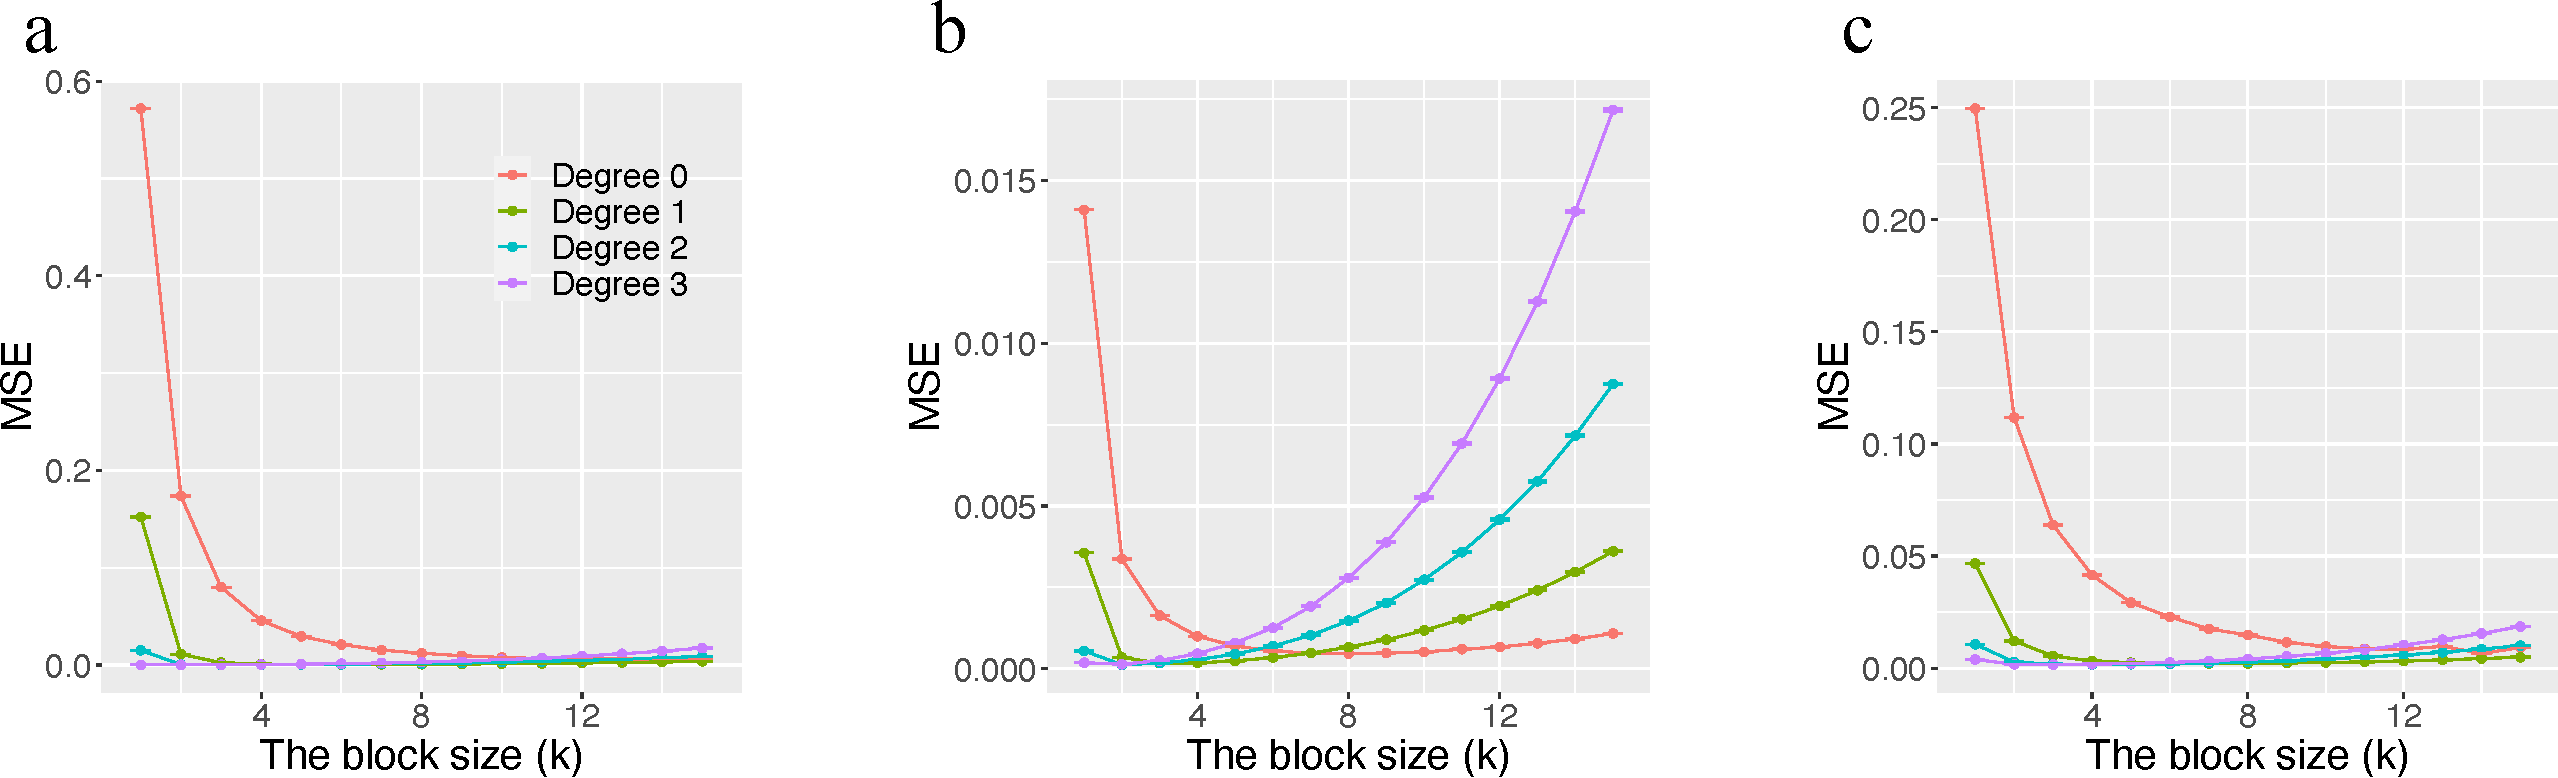
\includegraphics[width =.8\textwidth]{deg.pdf}    
    \caption{MSE comparison versus the number of blocks for different polynomial approximation. Panels a-c show the results under the models 1-3 respectively.}
    \label{fig:degk}
    \vspace{-.2cm}
\end{figure}

The second experiment compares our method ({\bf \small Borda Count}) with several popular alternative methods: (a) Spectral method ({\bf \small Spectral})~\citep{xu2018rates} that performs universal singular value thresholding~\citep{chatterjee2015matrix} on the unfolded tensor; (b) Least square estimation ({\bf \small LSE})~\cite{balasubramanian2021nonparametric}, which solves the optimization problem \eqref{eq:lseopt} with constant block approximation ($\ell = 0$)~\citep{gao2016optimal}; (c) Our {\bf \small Borda Count} algorithm. We choose degree-2 polynomial approximation as our theorems suggested, and 
vary tensor dimension $d\in\{10,\ldots,100\}$ under each model specification. We choose the block number for {\bf \small Borda Count} and {\bf \small LSE}, which achieves the best performance based on the intuition in our theorems and Figure~\ref{fig:degk}.  Similarly, we set the threshold value that obtains the best performance for {\bf \small Spectral}. 



\begin{figure}[htp]
    \centering
    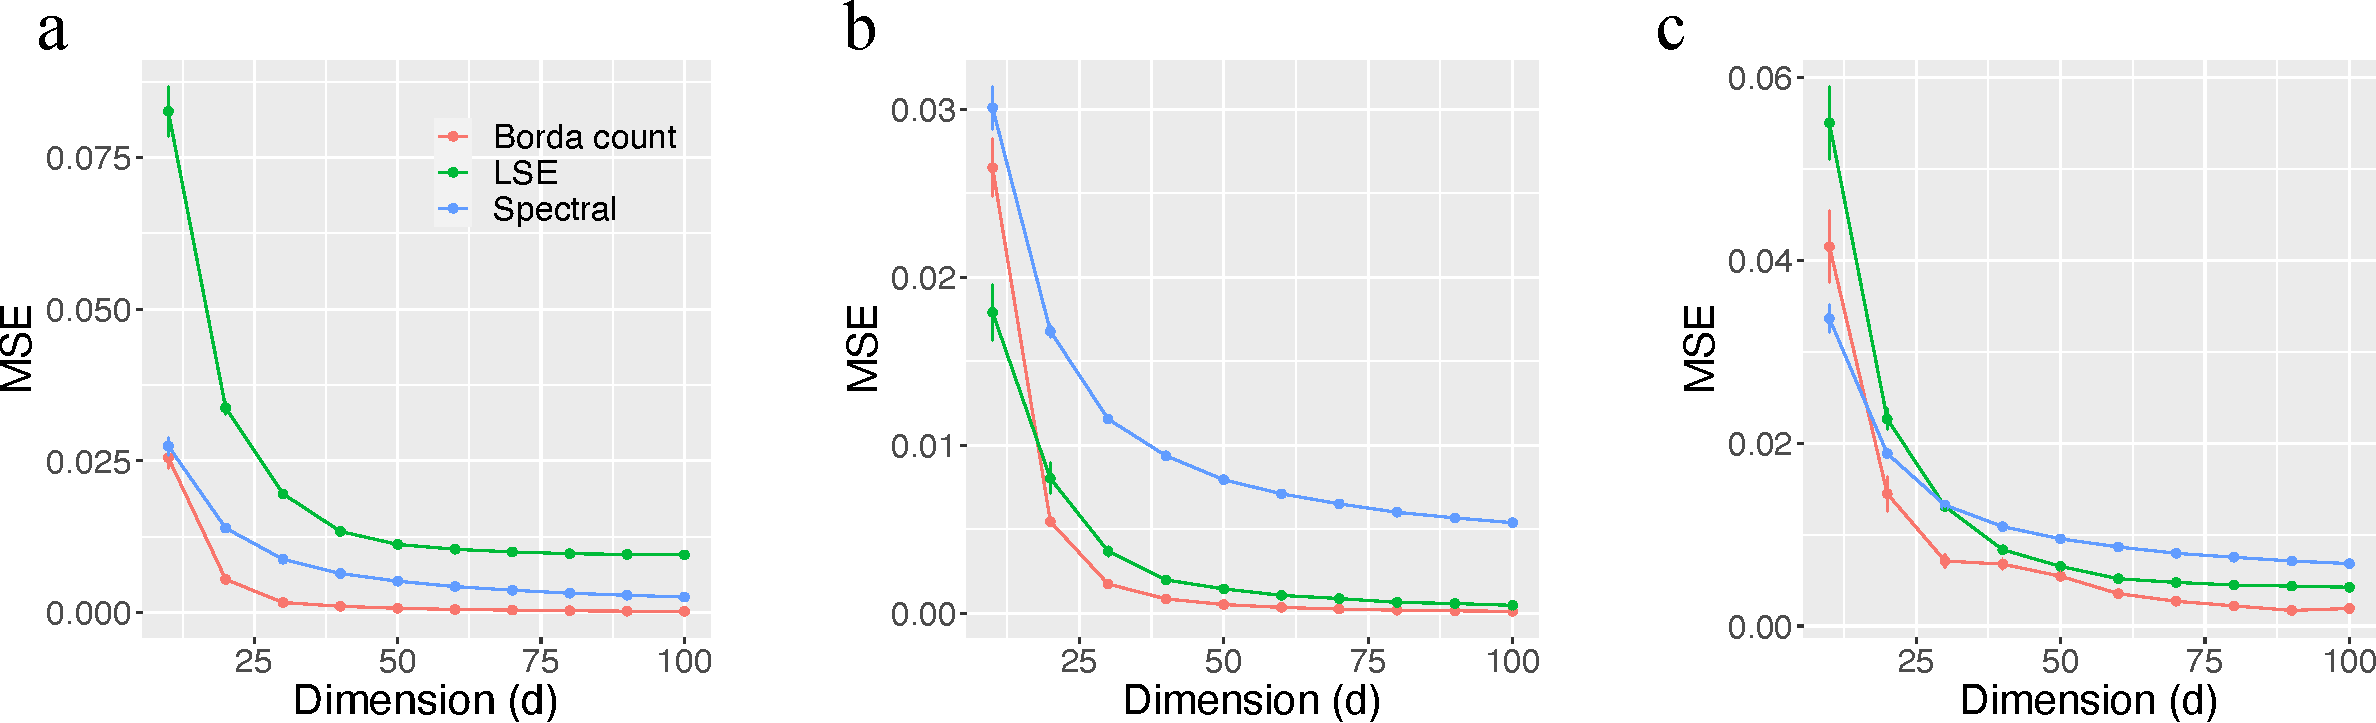
\includegraphics[width = .8\textwidth]{alt.pdf}    
    \caption{MSE comparison of different methods versus tensor dimension. Panels a-c show the results under models 1-3 respectively. }
    \label{fig:method}
    \vspace{-.2cm}
\end{figure}



Figure~\ref{fig:method} shows that our algorithm {\bf \small Borda Count} achieves the best performance in all scenarios as the tensor dimension increases. The poor performance of {\bf \small Spectral} can be explained by the loss of multilinear structure in the tensor unfolding procedure. The sub-optimality of {\bf \small LSE} is possibly due to its limits in both statistics and computations. Statistically, our theorems have shown that constant block approximation has sub-optimal rates compared to polynomial approximation for higher-order tensors. Computationally, the least square optimization~\eqref{eq:lseopt} is highly non-convex and computationally unstable. The outperformance of {\bf \small Borda count} demonstrates the efficacy of our method.


\vspace{-.2cm}
\section{Application to Chicago crime data}\label{sec:app}
\vspace{-.2cm}
 Chicago crime dataset consists of crime counts reported in the city of Chicago, ranging from January 1st, 2001 to December 11th, 2017. The observed tensor is an order-3 tensor with entries representing the log counts of crimes from 24 hours, 77 community areas, and 32 crime types. We apply our Borda Count method to Chicago crime dataset. Because the data tensor is asymmetric, we allow different number of blocks across the three modes. Cross validation result suggests the $(k_1,k_2,k_3)=(6,4,10)$, representing the block number for crime hours, community areas, and crime types, respectively.

We first investigate the four clustered community areas obtained from our Borda Count algorithm.  Figure~\ref{fig:area}(b) shows the four areas overlaid on a map of Chicago. Interestingly, we find that the clusters conform the actual locations even though our algorithm did not take any geographic information such as longitude or latitude as inputs. In addition, we compare the cluster patterns with benchmark results based on homicides- and shooting incidents-maps in Chicago shown in Figure~\ref{fig:area}(a). We find that our clusters share similar geographical patterns with Figure~\ref{fig:area}(a). The benchmark Figure~\ref{fig:area}(a) covers only homicides and shooting incidents in 2020, whereas our result in Figure~\ref{fig:area}(b) considers 32 crime types across 2001-2017. The results demonstrate the power of our approach in detecting meaningful pattern from tensor data. 
\begin{figure}[h]
    \centering
    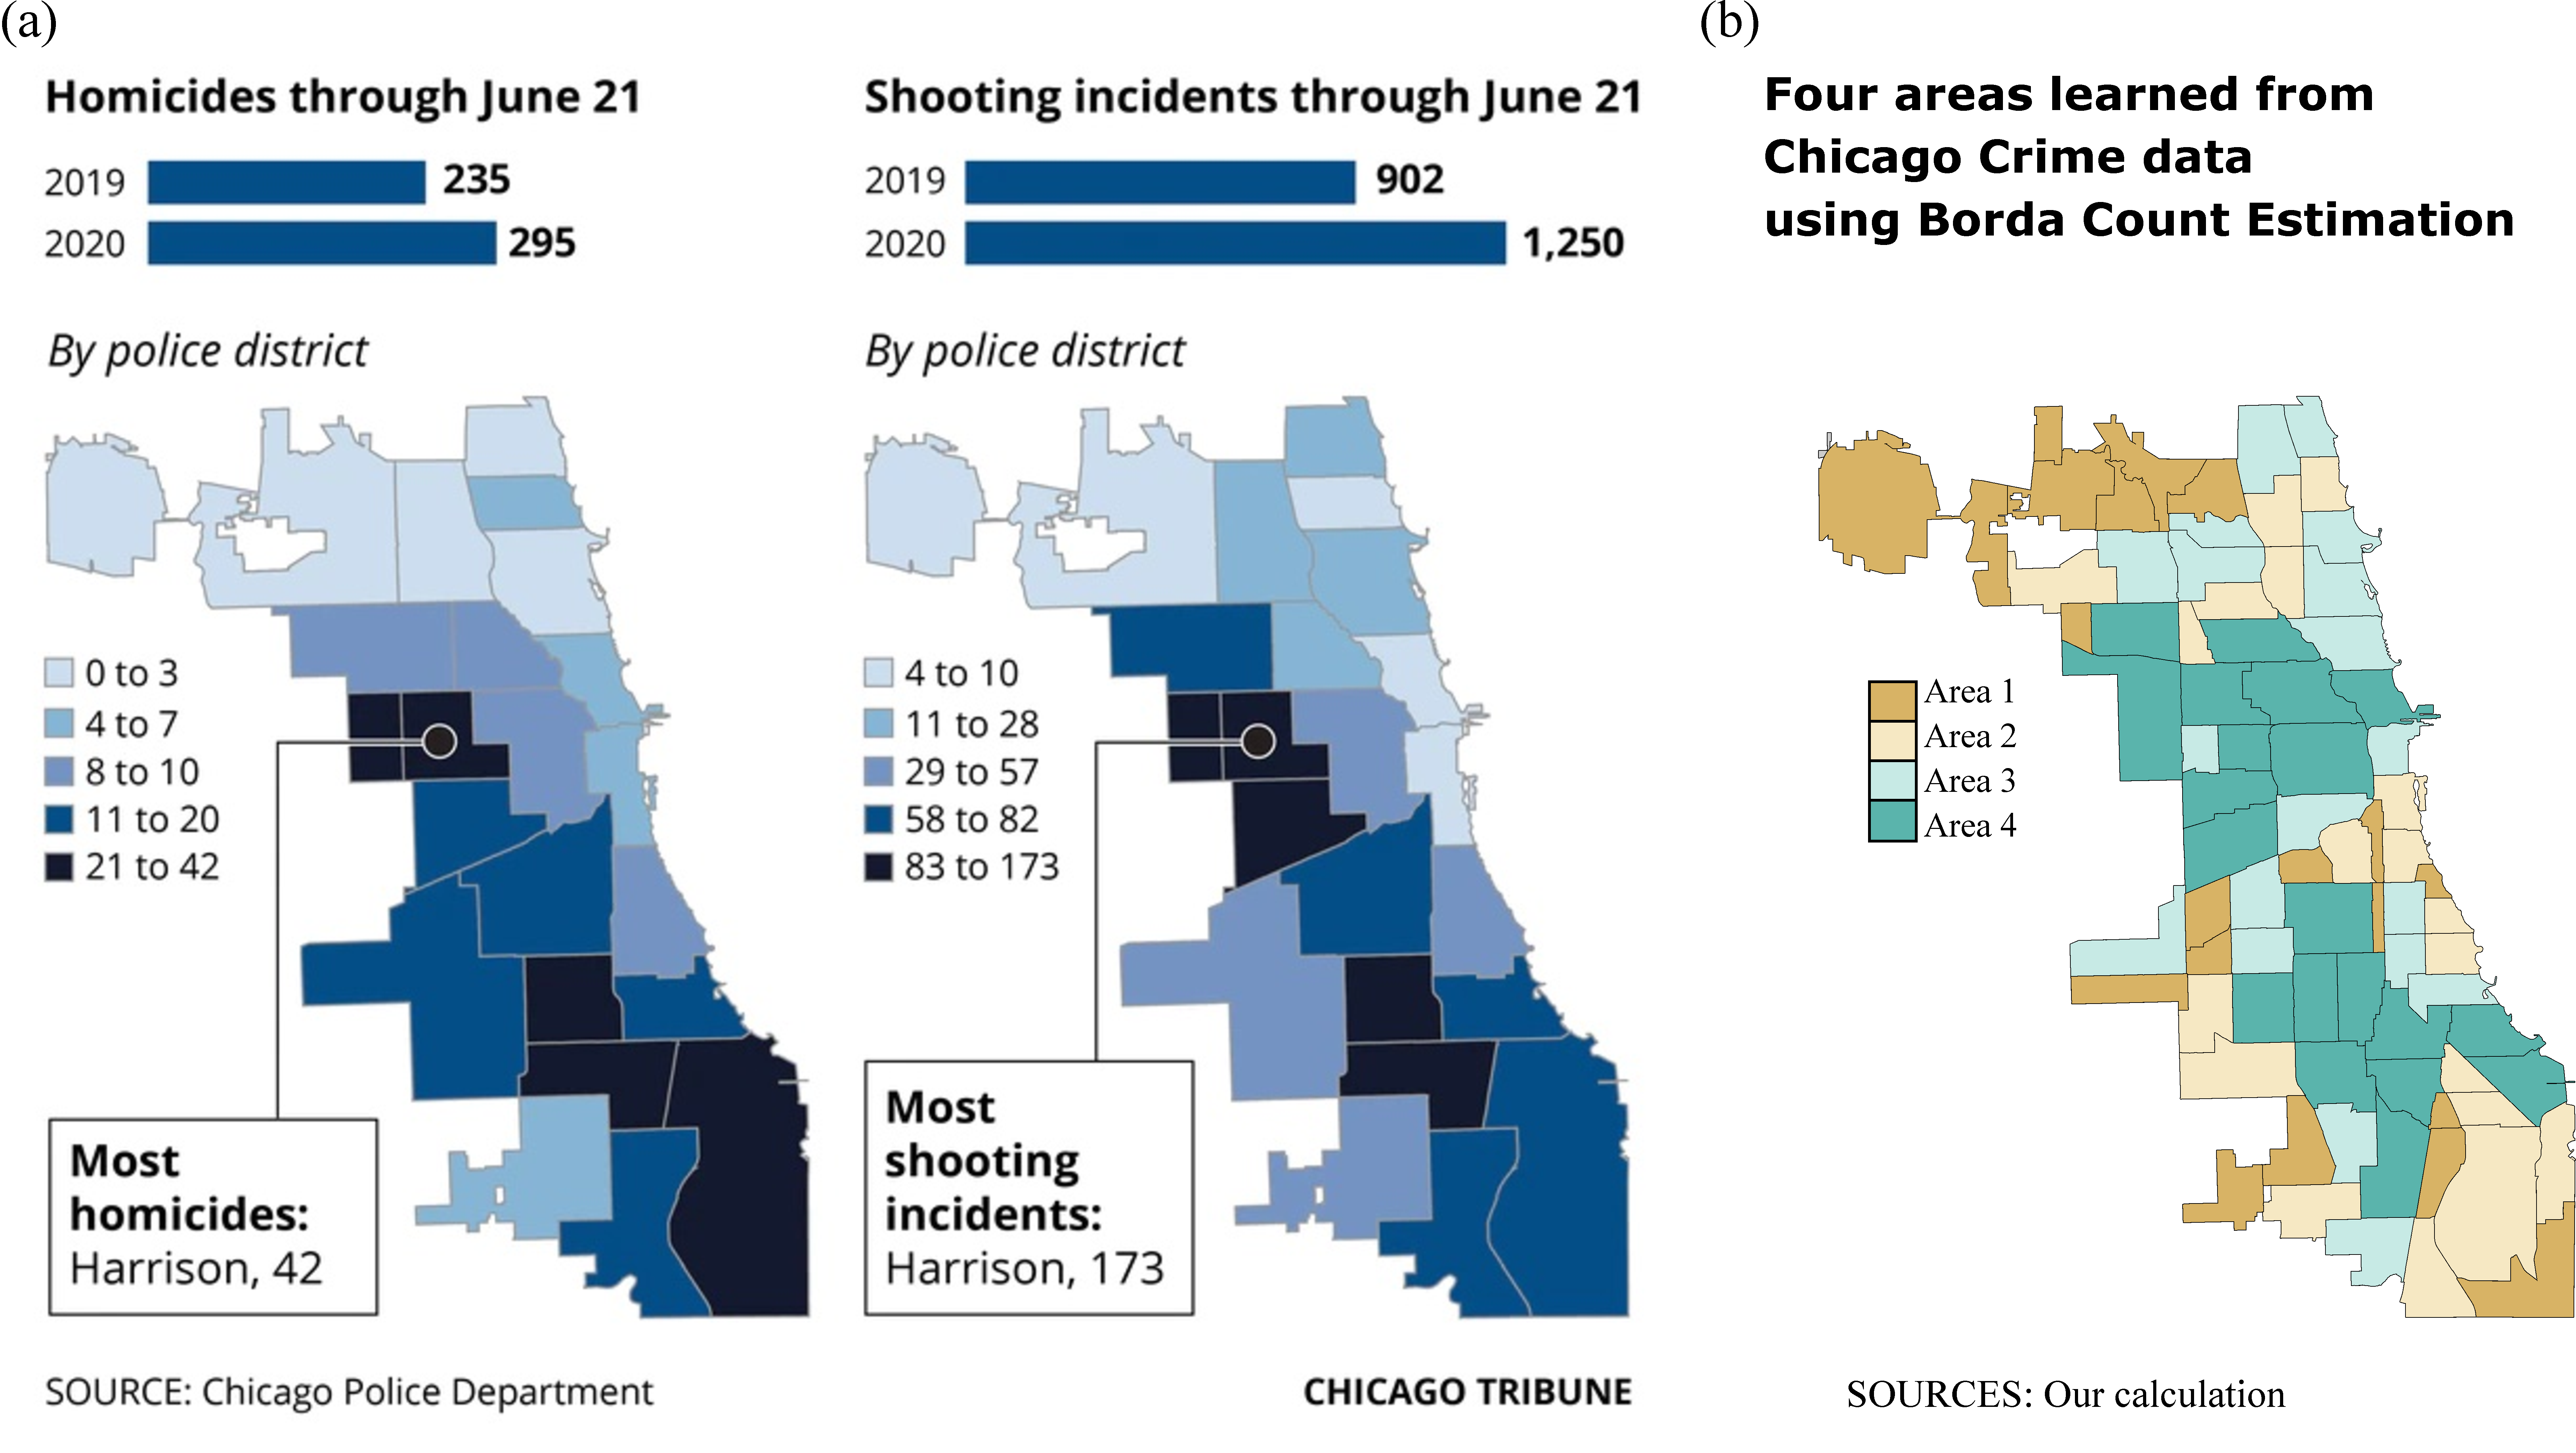
\includegraphics[width = .7\textwidth]{crimecompare.pdf}
    \caption{Chicago crime maps. Figure(a) shows homicides and shooting incidents in community areas in Chicago. This figure is from \textit{Chicago Tribune} article in 2020 \citep{Jeremy.2020}. Figure(b) shows the four areas estimated by our Borda Count algorithm. }
    \label{fig:area}
    \vspace{-.4cm}
\end{figure}
% \fixme{Miaoyan}{change ``Source; authors' calculation'' ``Sources: our calculation''.}


Then, we examine the denoised signal tensor obtained from our method and analyze the trends between crime types and crime hours by the four community areas in Figure~\ref{fig:area}(b). Figure~\ref{fig:crimeA} shows the averaged log counts of crimes according to crime types and crime hours by four areas. We find that the major difference among four areas is the crime rates. Area 4 has the highest crime rates,  and the crime rates monotonically decrease from Area 4 to Area 1. The variation in crime rates across hour and type, nevertheless, exhibits similarity among the four areas. For example, Figure~\ref{fig:crimeA} shows that the number of crimes increases hourly from 8 p.m., peaks at night hours, and then drops to the lowest at 6 p.m. 
The identified similarities and differences among the four community areas highlight the interpretability of our method in real data.
\begin{figure}[h]
    \centering
    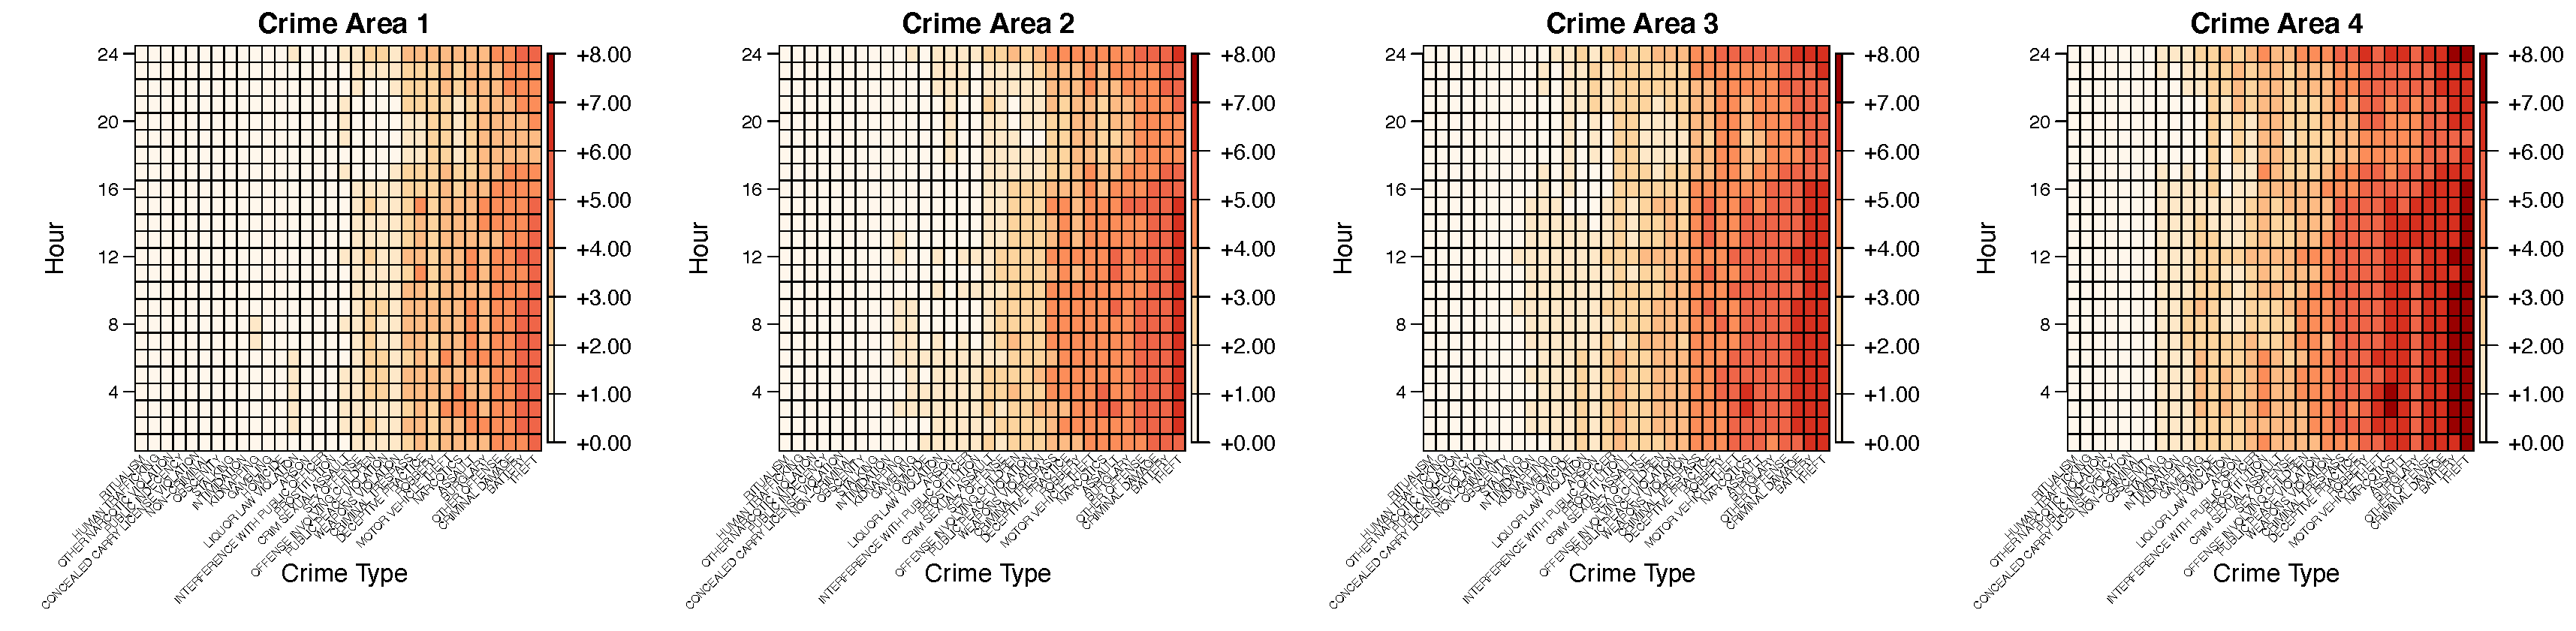
\includegraphics[width = \textwidth]{CrimeAn.pdf}
    \caption{Averaged log counts of crimes according to crime types, hours, and the four areas estimated by our Borda Count algorithm. We plot the estimated signal tensor entries averaged within four areas in the heatmap.}
    \label{fig:crimeA}
    \vspace{-.4cm}
\end{figure}

Finally, we compare the block-wise constant approximation versus block-wise degree-2 polynomial approximation. We assess the goodness-of-fit by considering the hypothesis testing
\begin{align}
    H_0 \colon \Theta \text{ is a block-wise constant tensor} \ \text{ vs. } \ H_1\colon \Theta \text{ is a block-wise polynomial degree-2 tensor}.
\end{align}
Notice that the class of block-wise constant tensors is nested within that of block-wise polynomial degree-2 tensors. Therefore, we perform a F-test considering the degree of freedom of each model. The degree of freedom of $H_0$ is the number of total blocks, $6\times 4\times 10$. The degree of $H_1$ is $10\times6\times 4\times 10$ because degree-2 polynomials have 10 times more coefficients than the constant block model. The obtained F-statistics from Chicago crime dataset is 19.63 with $p$-value is $<10^{-3}$. The result provides the significant evidence for the validity of the polynomial approximation. 
We emphasize that our method does not necessarily assume the block structure. We present F-test result as an evidence supporting our premises that permuted smooth tensor model with polynomial approximation performs better than common tensor block models in this application. 

\vspace{-.2cm}
\section{Conclusion}\label{sec:con}
\vspace{-.2cm}
We have developed permuted smooth tensor model and estimation methods with theoretical guarantees. 
%An optimal error bound for the least square estimation is established based on block-wise polynomial approximation. Borda count estimation with polynomial algorithm is provided with the same convergence rate under $\beta$-monotonicity. 
The efficacy of our procedure is demonstrated through both simulations and analysis of Chicago crime dateset. 



% Acknowledgements should go at the end, before appendices and references

%\acks{We would like to acknowledge support for this project from the National Science Foundation (NSF grant IIS-9988642) and the Multidisciplinary Research Program of the Department of Defense (MURI N00014-00-1-0637). }

% Manual newpage inserted to improve layout of sample file - not
% needed in general before appendices/bibliography.



% Note: in this sample, the section number is hard-coded in. Following
% proper LaTeX conventions, it should properly be coded as a reference:

%In this appendix we prove the following theorem from
%Section~\ref{sec:textree-generalization}:

\section*{Acknowledgements}
This research is supported in part by NSF grant DMS- 1915978, NSF DMS-2023239, and Wisconsin Alumni Research Foundation.


\bibliographystyle{plain}
\bibliography{tensor_wang}
%%%%%%%%%%%%%%%%%%%%%%%%%%%%%%%%%%%%%%%%%%%%%%%%%%%%%%%%%%%%
% \section*{Checklist}

% %%% BEGIN INSTRUCTIONS %%%
% The checklist follows the references.  Please
% read the checklist guidelines carefully for information on how to answer these
% questions.  For each question, change the default \answerTODO{} to \answerYes{},
% \answerNo{}, or \answerNA{}.  You are strongly encouraged to include a {\bf
% justification to your answer}, either by referencing the appropriate section of
% your paper or providing a brief inline description.  For example:
% \begin{itemize}
%   \item Did you include the license to the code and datasets? \answerYes{}
%   \item Did you include the license to the code and datasets? \answerNo{The code and the data are proprietary.}
%   \item Did you include the license to the code and datasets? \answerNA{}
% \end{itemize}
% Please do not modify the questions and only use the provided macros for your
% answers.  Note that the Checklist section does not count towards the page
% limit.  In your paper, please delete this instructions block and only keep the
% Checklist section heading above along with the questions/answers below.
% %%% END INSTRUCTIONS %%%

% \begin{enumerate}

% \item For all authors...
% \begin{enumerate}
%   \item Do the main claims made in the abstract and introduction accurately reflect the paper's contributions and scope?
%     \answerYes{} See Section~\ref{sec:int}, {\bf Contributions.}
%   \item Did you describe the limitations of your work?
%     \answerYes{} We provide the limitation of the least square estimation in  Section~\ref{sec:borda}
%   \item Did you discuss any potential negative societal impacts of your work?
%     \answerNA{} This work does not present any foreseeble societal consequence
%   \item Have you read the ethics review guidelines and ensured that your paper conforms to them?
%     \answerYes{}
% \end{enumerate}

% \item If you are including theoretical results...
% \begin{enumerate}
%   \item Did you state the full set of assumptions of all theoretical results?
%     \answerYes{} The assumptions for main Theorems are fully state.
% 	\item Did you include complete proofs of all theoretical results?
%     \answerNo{}
% \end{enumerate}

% \item If you ran experiments...
% \begin{enumerate}
%   \item Did you include the code, data, and instructions needed to reproduce the main experimental results (either in the supplemental material or as a URL)?
%     \answerNo{}
%   \item Did you specify all the training details (e.g., data splits, hyperparameters, how they were chosen)?
%     \answerYes{} Training procedures are described in Section~\ref{sec:sim}
% 	\item Did you report error bars (e.g., with respect to the random seed after running experiments multiple times)?
%     \answerYes{} Error bars are provided in all Figures
% 	\item Did you include the total amount of compute and the type of resources used (e.g., type of GPUs, internal cluster, or cloud provider)?
%     \answerNo{}
% \end{enumerate}

% \item If you are using existing assets (e.g., code, data, models) or curating/releasing new assets...
% \begin{enumerate}
%   \item If your work uses existing assets, did you cite the creators?
%     \answerYes{} Data source has been cited in Section~\ref{sec:app}
%   \item Did you mention the license of the assets?
%     \answerNA{} No license available for teh assets used in this work.
%   \item Did you include any new assets either in the supplemental material or as a URL?
%     \answerTODO{}
%   \item Did you discuss whether and how consent was obtained from people whose data you're using/curating?
%     \answerNA{} The datasets are publicly available.
%   \item Did you discuss whether the data you are using/curating contains personally identifiable information or offensive content?
%     \answerNA{} No personally identifiable information is included in the datsets.
% \end{enumerate}

% \item If you used crowdsourcing or conducted research with human subjects...
% \begin{enumerate}
%   \item Did you include the full text of instructions given to participants and screenshots, if applicable?
%     \answerNA{} This work does not involve human subjects.
%   \item Did you describe any potential participant risks, with links to Institutional Review Board (IRB) approvals, if applicable?
%     \answerNA{} This work does not involve potential participant risk
%   \item Did you include the estimated hourly wage paid to participants. and the total amount spent on participant compensation?
%     \answerNA{} This work does not involve participants.
% \end{enumerate}

% \end{enumerate}

%%%%%%%%%%%%%%%%%%%%%%%%%%%%%%%%%%%%%%%%%%%%%%%%%%%%%%%%%%%%


\end{document}